\documentclass[11pt]{article}
\usepackage[margin=0.8in]{geometry}
\usepackage{amsmath,amssymb,graphicx,hyperref}
\setlength{\parindent}{0pt}\setlength{\parskip}{4pt}
\setlength{\emergencystretch}{3em}
\begin{document}
{\Large Actual cofactor equations force a full nonzero norm}\par
2026-11-13. Unsigned producer evidence [pcc:unverified].

The actual reduced coefficient cofactor equations now imply
\[
 (C\alpha\,F)^2-f(C\beta\,H)^2=Cc\,G,\qquad c\ne0.
\]
No norm identity, nonzero-normalization oracle, numerical rank or coordinate
oracle is supplied to the final theorem. The prior actual branch construction
derives its matrix guards. Suitable $F,H,V$ and the cofactor equations are
still inputs. Frozen source \path{5e7f9bb5c}; \path{NormCertificateRecovery}.

\textbf{Exact hypotheses.} Over a field: $F,H,G$ monic, $\deg H>0$,
$\deg H+1<\deg F$, $UF+V(fH)=1$, $F(q)\ne0$, $\alpha\ne0$,
$\alpha F(q)-y\beta H(q)=0$, and
\[
 2\deg F\le\deg G,\qquad \deg f+2\deg H\le\deg G.
\]
For each $j<\deg G$, pair the actual reduced residual coefficient matrix
$Q_{{\rm red},j}$ with the adjugate of the actual quotient-moment matrix
$S_{\rm red}$. All these pairings must be zero. The norm identity itself is
not among the assumptions [pcc:unverified].

\textbf{Noncircular extraction.} A nonzero diagonal cofactor gives an actual
nonzero adjugate column. The matrix-adjugate identity places it in the actual
kernel. The exact radical line makes it a nonzero scalar multiple of the
reduced candidate polynomial direction. Rank-one adjugate factorization and
nonzero scaling transfer all pairings to the actual quadratic residuals.
Public branch insertion gives every residual coefficient of the original
norm. The degree bounds and coefficient extensionality reconstruct the full
polynomial [pcc:unverified].

\begin{center}
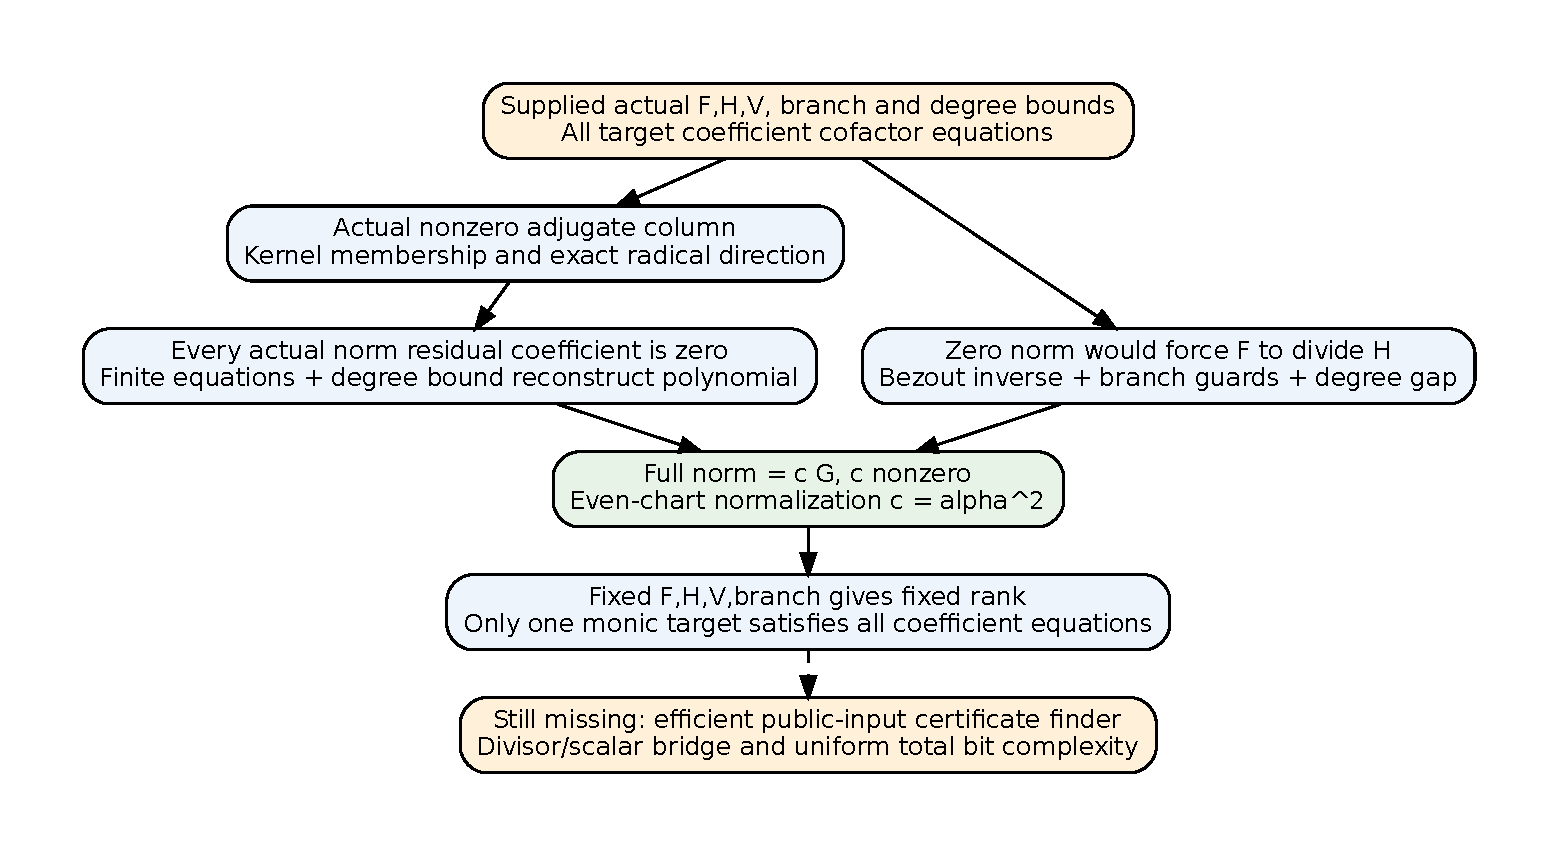
\includegraphics[width=0.95\linewidth,height=0.30\textheight,keepaspectratio]{recovery.pdf}
\end{center}

\textbf{Nonzero normalization.} The branch guards imply $\beta\ne0$. A zero
norm would give $fH^2$ as a constant multiple of $F^2$. Multiply the Bezout
identity by $H$: then $F\mid H$, contradicting the degree gap. Hence the
reconstructed scalar is nonzero. It is a polynomial normalization, not the
secret discrete logarithm [pcc:unverified].

\newpage
{\Large Exact normalization, falsification control and remaining finder}\par

\textbf{Even chart.} If $\deg F=\deg H+2$, $\deg f\le3$ and
$\deg G=2\deg F$, the lower norm term has degree strictly below $2\deg F$.
Monicity makes the top coefficient exactly $\alpha^2$. Thus the actual
normalization is $c=\alpha^2\ne0$. The old normOfWitnessLine theorem, which
already assumes a norm identity, is not used circularly [pcc:unverified].

\textbf{Target control.} Fixed $F,H,V,q,y$ give a fixed reduced moment matrix;
it does not depend on $G$. A fixed nonzero norm has at most one monic target.
Combining this uniqueness lemma with actualNonzeroNorm, at most one monic
$G$ can satisfy all actual cofactor equations under the stated bounds.
Rank alone is therefore an insufficient experimental gate [pcc:unverified].

\textbf{Native regression.} On the existing F17 example, both fixed supports
retain the same curve, branch $q=0,y=6$, monic degree 6 and distinct rational
nonzero-$y$ lifts. The same reduced matrix has rank 4 and determinant 0.
The changed set replaces 13 by 7; it is wrong for this certificate, not asserted
globally unsatisfiable. One artifact invocation contains two controls
[pcc:unverified].

\begin{center}\small
\begin{tabular}{lcl}
Support & Rank & Cofactor pairings modulo 17\\\hline
0,3,5,6,10,13 & 4 & 0,0,0,0,0,0\\
0,3,5,6,7,10 & 4 & 0,12,4,12,16,5
\end{tabular}\end{center}

Pairings equal 2 times the actual norm residuals. Checked literal congruence,
Gaussian rank versus independent Leibniz determinant/adjugate, both adjugate
products, rational lifts and all chart guards. Three tests, strict clippy and
formatting pass. Native source \path{582e21bfb}, fixed-case contract
\path{ad3005105}; unsigned data \path{PCC-20261113-1aa548}. This is a finite
development regression, not timing, relation-yield or independent A/A evidence.

\begin{center}\small
\begin{tabular}{ll}
Exact component & Declaration in \path{NormCertificateRecovery}\\\hline
Actual residual coefficients & \path{actualNormResidual}\\
Full nonzero norm & \path{actualNonzeroNorm}\\
Even-chart normalization & \path{actualNormalizedNorm}\\
Monic target uniqueness & \path{monicScalarTargetUnique}
\end{tabular}\end{center}

\textbf{Verification scope.} There are 16 new statements. Builds 001--005 all
pass with explicit exits; no new-module warning. Whole-study
tracked-source audit: 217 statements, 0 additional trusted axioms. The
import-inclusive fresh replay has a separate completion receipt. Exact source
bindings, logs and input hashes accompany this report. Producer checks do not
supply independent signed PCC standing. No solver, timing, paid experiment,
benchmark, leaderboard or ecdb row is added. Native clippy was initially
absent; installed the component. The globally ignored lockfile was tracked
before execution. No proof or native arithmetic check failed.

\textbf{Remaining obligations.} The polynomial certificate is now connected
to its full nonzero norm for this chart. Prime subgroup, rational factor-base
support, divisor/group relation and discrete-log recovery are additional
application obligations. Efficiently finding the supplied $F,H,V$ and target
cofactor equations remains the algorithmic gap. A sub-exponential claim needs
uniform total expected $\exp(o(\log r))$ work, including setup, rejected
attempts, relation yield, linear algebra and final recovery. A certificate
checker is not that finder. Reachability through the annotated jet completion
remains separate and unproved; its $H$ is not the norm polynomial by naming.

\textbf{Sources.} Prior branch, cofactor, extraction, norm and coefficient
sources; pinned polynomial monic/degree/divisibility APIs; existing F17 control.
KB unavailable. Standard algebra, no priority or algorithmic novelty claim.
Exact paths, source bindings and reproduction commands are in the README.
\end{document}
